\newpage
\section{Ablations for Section~\ref{sec:challenges-measuring}}
\label{sec:appendix_platt_experiments}

Here we present additional experiments for Section~\ref{sec:challenges-measuring}.
Recall that the experiments in section~\ref{sec:challenges-measuring} showed that binning underestimates the calibration error of a model---we focused on the $\ell_2\mbox{-CE}$ and selected bins so that each bin has an equal number of data points. Figure~\ref{fig:imagenet_lower_bound_l1} shows that binning is also unreliable at measuring the $\ell_1\mbox{-CE}$ on ImageNet---using more bins uncovers a higher calibration error than we would otherwise detect with fewer bins. Figure~\ref{fig:imagenet_lower_bound_l1_prob} shows that the same conclusion holds on ImageNet if we look at the $\ell_1\mbox{-CE}$ \emph{and} use an alternative approach to selecting bins used in~\cite{guo2017calibration} that we call \emph{equal-probability binning}. Here, the $B$ bins are selected to be $I_1 = [0, \frac{1}{B}], I_2 = (\frac{1}{B}, \frac{2}{B}], \dots, I_B = (\frac{B-1}{B}, 1]$. The experimental protocol is the same as in section~\ref{sec:challenges-measuring}.

\begin{figure}
     \centering
     \begin{subfigure}[b]{0.45\textwidth}
         \centering
         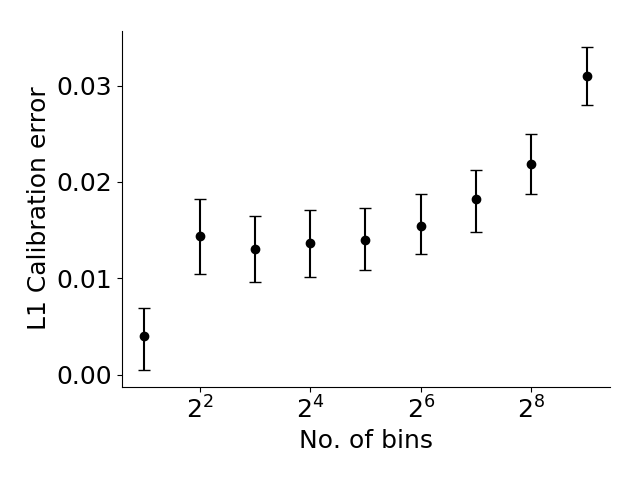
\includegraphics[width=\textwidth]{l1_lower_bound_imagenet_plot}
         \caption{ImageNet, $\ell_1\mbox{-CE}$}
         \label{fig:imagenet_lower_bound_l1}
     \end{subfigure}
     \hfill
     \begin{subfigure}[b]{0.45\textwidth}
         \centering
         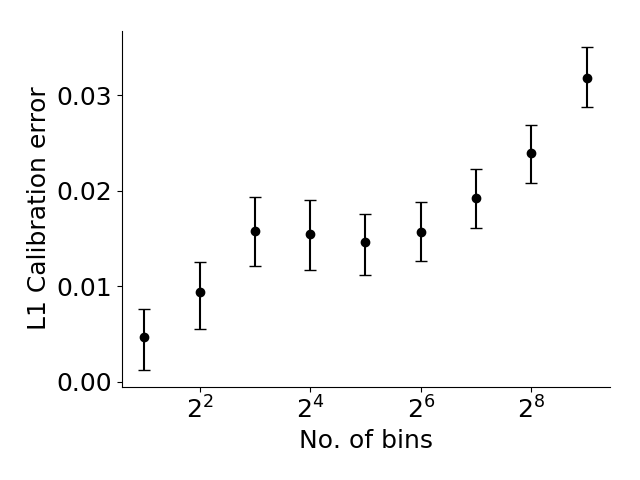
\includegraphics[width=\textwidth]{l1_lower_bound_imagenet_plot_prob_bin}
         \caption{ImageNet, $\ell_1\mbox{-CE}$, equal-probability binning}
         \label{fig:imagenet_lower_bound_l1_prob}
     \end{subfigure}
        \caption{
        Binned $\ell_1$ calibration errors of a recalibrated VGG-net model on ImageNet with $90\%$ confidence intervals. The binned calibration error increases as we increase the number of bins. This suggests that binning cannot be reliably used to measure the $\ell_1\mbox{-CE}$.
        }
        \label{fig:lower_bounds_l1_imagenet}
\end{figure}

We repeated both of these experiments on CIFAR-10 as well, and plot the results in Figure~\ref{fig:lower_bounds_l1_cifar}. Here the results are inconclusive because the error bars are large. This is because the CIFAR-10 dataset is smaller than ImageNet, and the accuracy of the CIFAR-10 model is 93.1\%, so the calibration error that we are trying to measure is much smaller.

\begin{figure}
     \centering
     \begin{subfigure}[b]{0.45\textwidth}
         \centering
         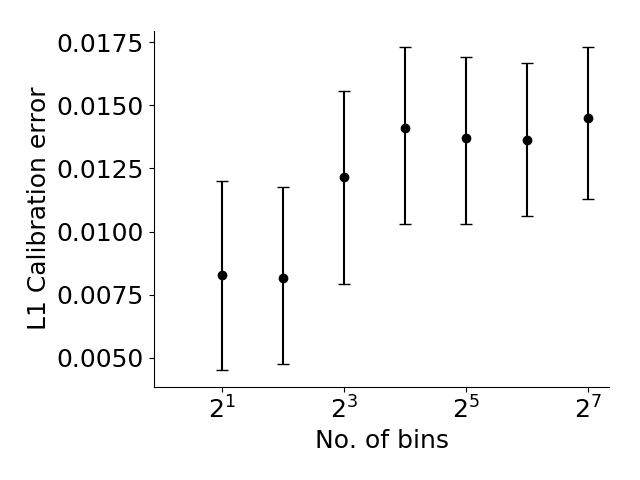
\includegraphics[width=\textwidth]{l1_lower_bound_cifar_plot}
         \caption{CIFAR-10, $\ell_1\mbox{-CE}$}
         \label{fig:cifar_lower_bound_l1}
     \end{subfigure}
     \hfill
     \begin{subfigure}[b]{0.45\textwidth}
         \centering
         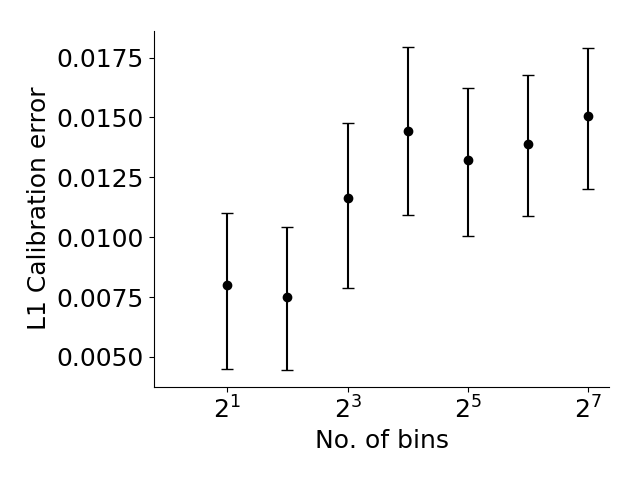
\includegraphics[width=\textwidth]{l1_lower_bound_cifar_plot_prob_bin}
         \caption{CIFAR-10, $\ell_1\mbox{-CE}$, equal-probability binning}
         \label{fig:cifar_lower_bound_l1_prob}
     \end{subfigure}
        \caption{
        Binned $\ell_1$ calibration errors of a recalibrated VGG-net model on CIFAR-10 with $90\%$ confidence intervals. The results are not as conclusive here because the error bars are large, however it seems to suggest that the binned calibration error increases as we increase the number of bins.
        }
        \label{fig:lower_bounds_l1_cifar}
\end{figure}

We provide details on the dataset split for CIFAR-10. For CIFAR-10, we used a VGG16 model and split the test set into 3 sets of size $(1000, 1000, 8000)$, where used the first set of data to recalibrate the model using Platt scaling, the second to select the binning scheme, and the third to measure the binned calibration error. As stated in the main body of the paper, for ImageNet we used a split of $(20000, 5000, 25000)$
